
\documentclass[11pt,a4paper,UTF8]{book}

\usepackage[T1]{fontenc}
\usepackage[utf8]{inputenc}
\usepackage{authblk}

\usepackage{ctex} %導入中文包

\setCJKmainfont{LiHei Pro}
\setCJKsansfont{LiHei Pro}
\setCJKmonofont{LiHei Pro}

%\usepackage{ulem}
\usepackage{tocvsec2}

\usepackage{tabularx}
\usepackage{booktabs} 
\usepackage{multirow}
\usepackage{bbding}
\usepackage{float}
\usepackage{xspace}
\usepackage[none]{hyphenat}

\usepackage{graphicx}
\usepackage{subfigure}
\usepackage{pifont}

\usepackage{hyperref}  %製作pdf的目錄
\usepackage{subfiles} %使用多文件方式進行

\usepackage{geometry} %設置頁邊距的包
\geometry{left=2.5cm,right=2cm,top=2.54cm,bottom=2.54cm} %設置書籍的頁邊距

\usepackage{url}
\hypersetup{hidelinks, %去紅框
	colorlinks=true,
	allcolors=black,
	pdfstartview=Fit,
	breaklinks=true
}

% 調整itemlist中的行間距
\usepackage{enumitem}
\setenumerate[1]{itemsep=0pt,partopsep=0pt,parsep=\parskip,topsep=5pt}
\setitemize[1]{itemsep=0pt,partopsep=0pt,parsep=\parskip,topsep=5pt}
\setdescription{itemsep=0pt,partopsep=0pt,parsep=\parskip,topsep=5pt}

% 超鏈接樣式設置
\usepackage{hyperref}
\hypersetup{
	colorlinks=true,
	linkcolor=blue,
	filecolor=blue,
	urlcolor=blue,
	citecolor=cyan,
}

\usepackage{indentfirst}

\usepackage{listings}
\usepackage[usenames,dvipsnames,svgnames, x11names]{xcolor}

\usepackage[most]{tcolorbox}

%展示代碼
\definecolor{mygreen}{rgb}{0,0.6,0}
\definecolor{mygray}{rgb}{0.5,0.5,0.5}
\definecolor{mymauve}{rgb}{0.58,0,0.82}
\definecolor{keywordcolor}{rgb}{0.8,0.1,0.5}
\definecolor{webgreen}{rgb}{0,.5,0}
\definecolor{bgcolor}{rgb}{0.92,0.92,0.92}

%定義CMake
\lstdefinelanguage{CMake}
{morekeywords={
		cmake\_minimum\_required,
		project,
		add\_executable,
		add\_library,
		target\_link\_libraries,
		cmake\_parse\_arguments,
		cmake\_language,
		set, unset,
		option,
		string,
		list,
		math,
		message,
		if, elseif, else, endif,
		mark\_as\_advanced,
		foreach, endforeach,
		while, endwhile,
		add\_subdirectory, include, return, include\_gurad,
		function, endfunction,
		macro, endmacro,
		find\_package,
		cmake\_push\_check\_state,
		cmake\_pop\_check\_state,
		cmake\_reset\_check\_state,
		add\_test,
		set\_tests\_properties, 
		check\_c\_source\_runs,
		check\_cxx\_source\_runs,
		check\_fortran\_source\_runs,
		check\_source\_runs,
		check\_compiler\_flag,
		check\_c\_compiler\_flag,
		check\_cxx\_compiler\_flag,
		check\_fortran\_compiler\_flag,
		check\_symbol\_exists,
		check\_cxx\_symbol\_exists,
		check\_linker\_flag,
		cmake\_policy,
		set\_property,
		get\_property,
		define\_property,
		get\_cmake\_property,
		set\_cmake\_property,
		set\_target\_properties,
		get\_target\_property,
		set\_directory\_properties,
		get\_directory\_property,
		set\_source\_files\_properties,
		get\_source\_file\_property,
		set\_tests\_properties,
		get\_tests\_property,
		get\_test\_property,
		cmake\_print\_properties,
		cmake\_print\_variables,
		variable\_watch,
		include\_guard,
		target\_link\_options,
		target\_compile\_definitions,
		target\_compile\_options,
		include\_directories,
		add\_definitions,
		remove\_definitions,
		add\_compile\_definitions,
		add\_compile\_options,
		link\_libraries,
		link\_directories,
		add\_link\_options,
		target\_include\_directories,
		target\_compile\_features,
		add\_custom\_command,
		add\_custom\_target,
		execute\_process,
		cmake\_path,
		get\_filename\_component,
		file,
		configure\_file,
		generate\_export\_header,
		export,
		find\_file,
		find\_library,
		find\_package,
		find\_program,
		pkg\_check\_modules,
		pkg\_search\_module,
		pkg\_get\_variable,
		add\_test,
		enable\_testing,
		set\_tests\_properties,
		site\_name,
		ctest\_empty\_binary\_directory,
		ctest\_start,
		ctest\_configure,
		ctest\_submit,
		ctest\_build,
		ctest\_memcheck,
		ctest\_upload,
		ctest\_test,
		gtest\_add\_tests,
		gtest\_discover\_tests,
		install,
		write\_basic\_package\_version\_file,
		configure\_package\_config\_file,
		cpack\_add\_component,
		cpack\_add\_install\_type,
		cpack\_add\_component\_group,
		ExternalProject\_Add,
		ExternalProject\_Add\_StepDependencies,
		ExternalProject\_Get\_Property,
		ExternalProject\_Add\_Step,
		FetchContent\_Declare,
		FetchContent\_GetProperties,
		FetchContent\_Populate,
		source\_group,
		target\_precompile\_headers,
		qt5\_wrap\_cpp,
		qt5\_wrap\_ui,
		qt5\_add\_resources,
		qt5\_add\_big\_resources,
		qt5\_add\_binary\_resources,
		qt5\_add\_translation,
		qt5\_create\_translation,
		compile\_definitions,
		add\_llvm\_component\_library,
		add\_llvm\_tool,
		llvm\_multisource,
		llvm\_test\_data,
	}, %定義關鍵字
	sensitive=false, %是否大小寫敏感
	morecomment=[l]{\#},
	morestring=[b]",
	morestring=[d]',
}

\lstdefinestyle{styleCXX}{
	language = C++,  
	backgroundcolor=\color{blue!3!white}, 
	%basicstyle = \footnotesize,  
	basicstyle      =   \zihao{-5}\ttfamily,
	numberstyle     =   \zihao{-5}\ttfamily,   
	%breakatwhitespace = false,    
	basewidth       =   0.5em,    
	breaklines = true,                 
	captionpos = b,                    
	commentstyle = \color{mygreen}\bfseries,
	%extendedchars = false,             
	frame =shadowbox, 
	framerule=0.5pt,
	%frameround = fttt,
	keepspaces=true,
	keywordstyle=\color{blue}\bfseries, % keyword style
	otherkeywords={string}, 
	numbers=left, 
	numbersep=5pt,
	numberstyle=\tiny\color{mygray},
	rulecolor=\color{black},         
	%showspaces=false,  
	%showstringspaces=false, 
	%showtabs=false,    
	%stepnumber=1,         
	stringstyle=\color{mymauve},        % string literal style
	tabsize=2,          
	columns         =   fixed,
	flexiblecolumns,                   
}

\tcbset{
	commandshell/.style={
		listing only,
		colback=black!75!white,
		colupper=white,
		lowerbox=ignored,
		listing options={
			language={bash},
			basicstyle=\ttfamily,
			columns = fixed,
			flexiblecolumns
		}
}}

\usepackage{tikz}

% URL 正確換行
% https://liam.page/2017/05/17/help-the-url-command-from-hyperref-to-break-at-line-wrapping-point/
\makeatletter
\def\UrlAlphabet{%
	\do\a\do\b\do\c\do\d\do\e\do\f\do\g\do\h\do\i\do\j%
	\do\k\do\l\do\m\do\n\do\o\do\p\do\q\do\r\do\s\do\t%
	\do\u\do\v\do\w\do\x\do\y\do\z\do\A\do\B\do\C\do\D%
	\do\E\do\F\do\G\do\H\do\I\do\J\do\K\do\L\do\M\do\N%
	\do\O\do\P\do\Q\do\R\do\S\do\T\do\U\do\V\do\W\do\X%
	\do\Y\do\Z}
\def\UrlDigits{\do\1\do\2\do\3\do\4\do\5\do\6\do\7\do\8\do\9\do\0}
\g@addto@macro{\UrlBreaks}{\UrlOrds}
\g@addto@macro{\UrlBreaks}{\UrlAlphabet}
\g@addto@macro{\UrlBreaks}{\UrlDigits}
\makeatother

% enable subsubsubsection
% from https://tex.stackexchange.com/questions/274212/correct-hierarchy-levels-of-pdf-bookmarks-for-custom-section-subsubsubsection
\usepackage[depth=3]{bookmark}
\setcounter{secnumdepth}{3}
\setcounter{tocdepth}{4}
\hypersetup{bookmarksdepth=4}

\makeatletter

\newcommand{\toclevel@subsubsubsection}{4}
\newcounter{subsubsubsection}[subsubsection]

\renewcommand{\thesubsubsubsection}{\thesubsubsection.\arabic{subsubsubsection}}

\newcommand{\subsubsubsection}{\@startsection{subsubsubsection}{4}{\z@}%
	{-3.25ex\@plus -1ex \@minus -.2ex}%
	{1.5ex \@plus .2ex}%
	{\normalfont\normalsize\bf\bfseries}}

\newcommand*{\l@subsubsubsection}{\@dottedtocline{4}{11em}{5em}}  

\newcommand{\subsubsubsectionmark}[1]{}
\makeatother

\begin{document}
%\maketitle

\begin{center}
\thispagestyle{empty}
%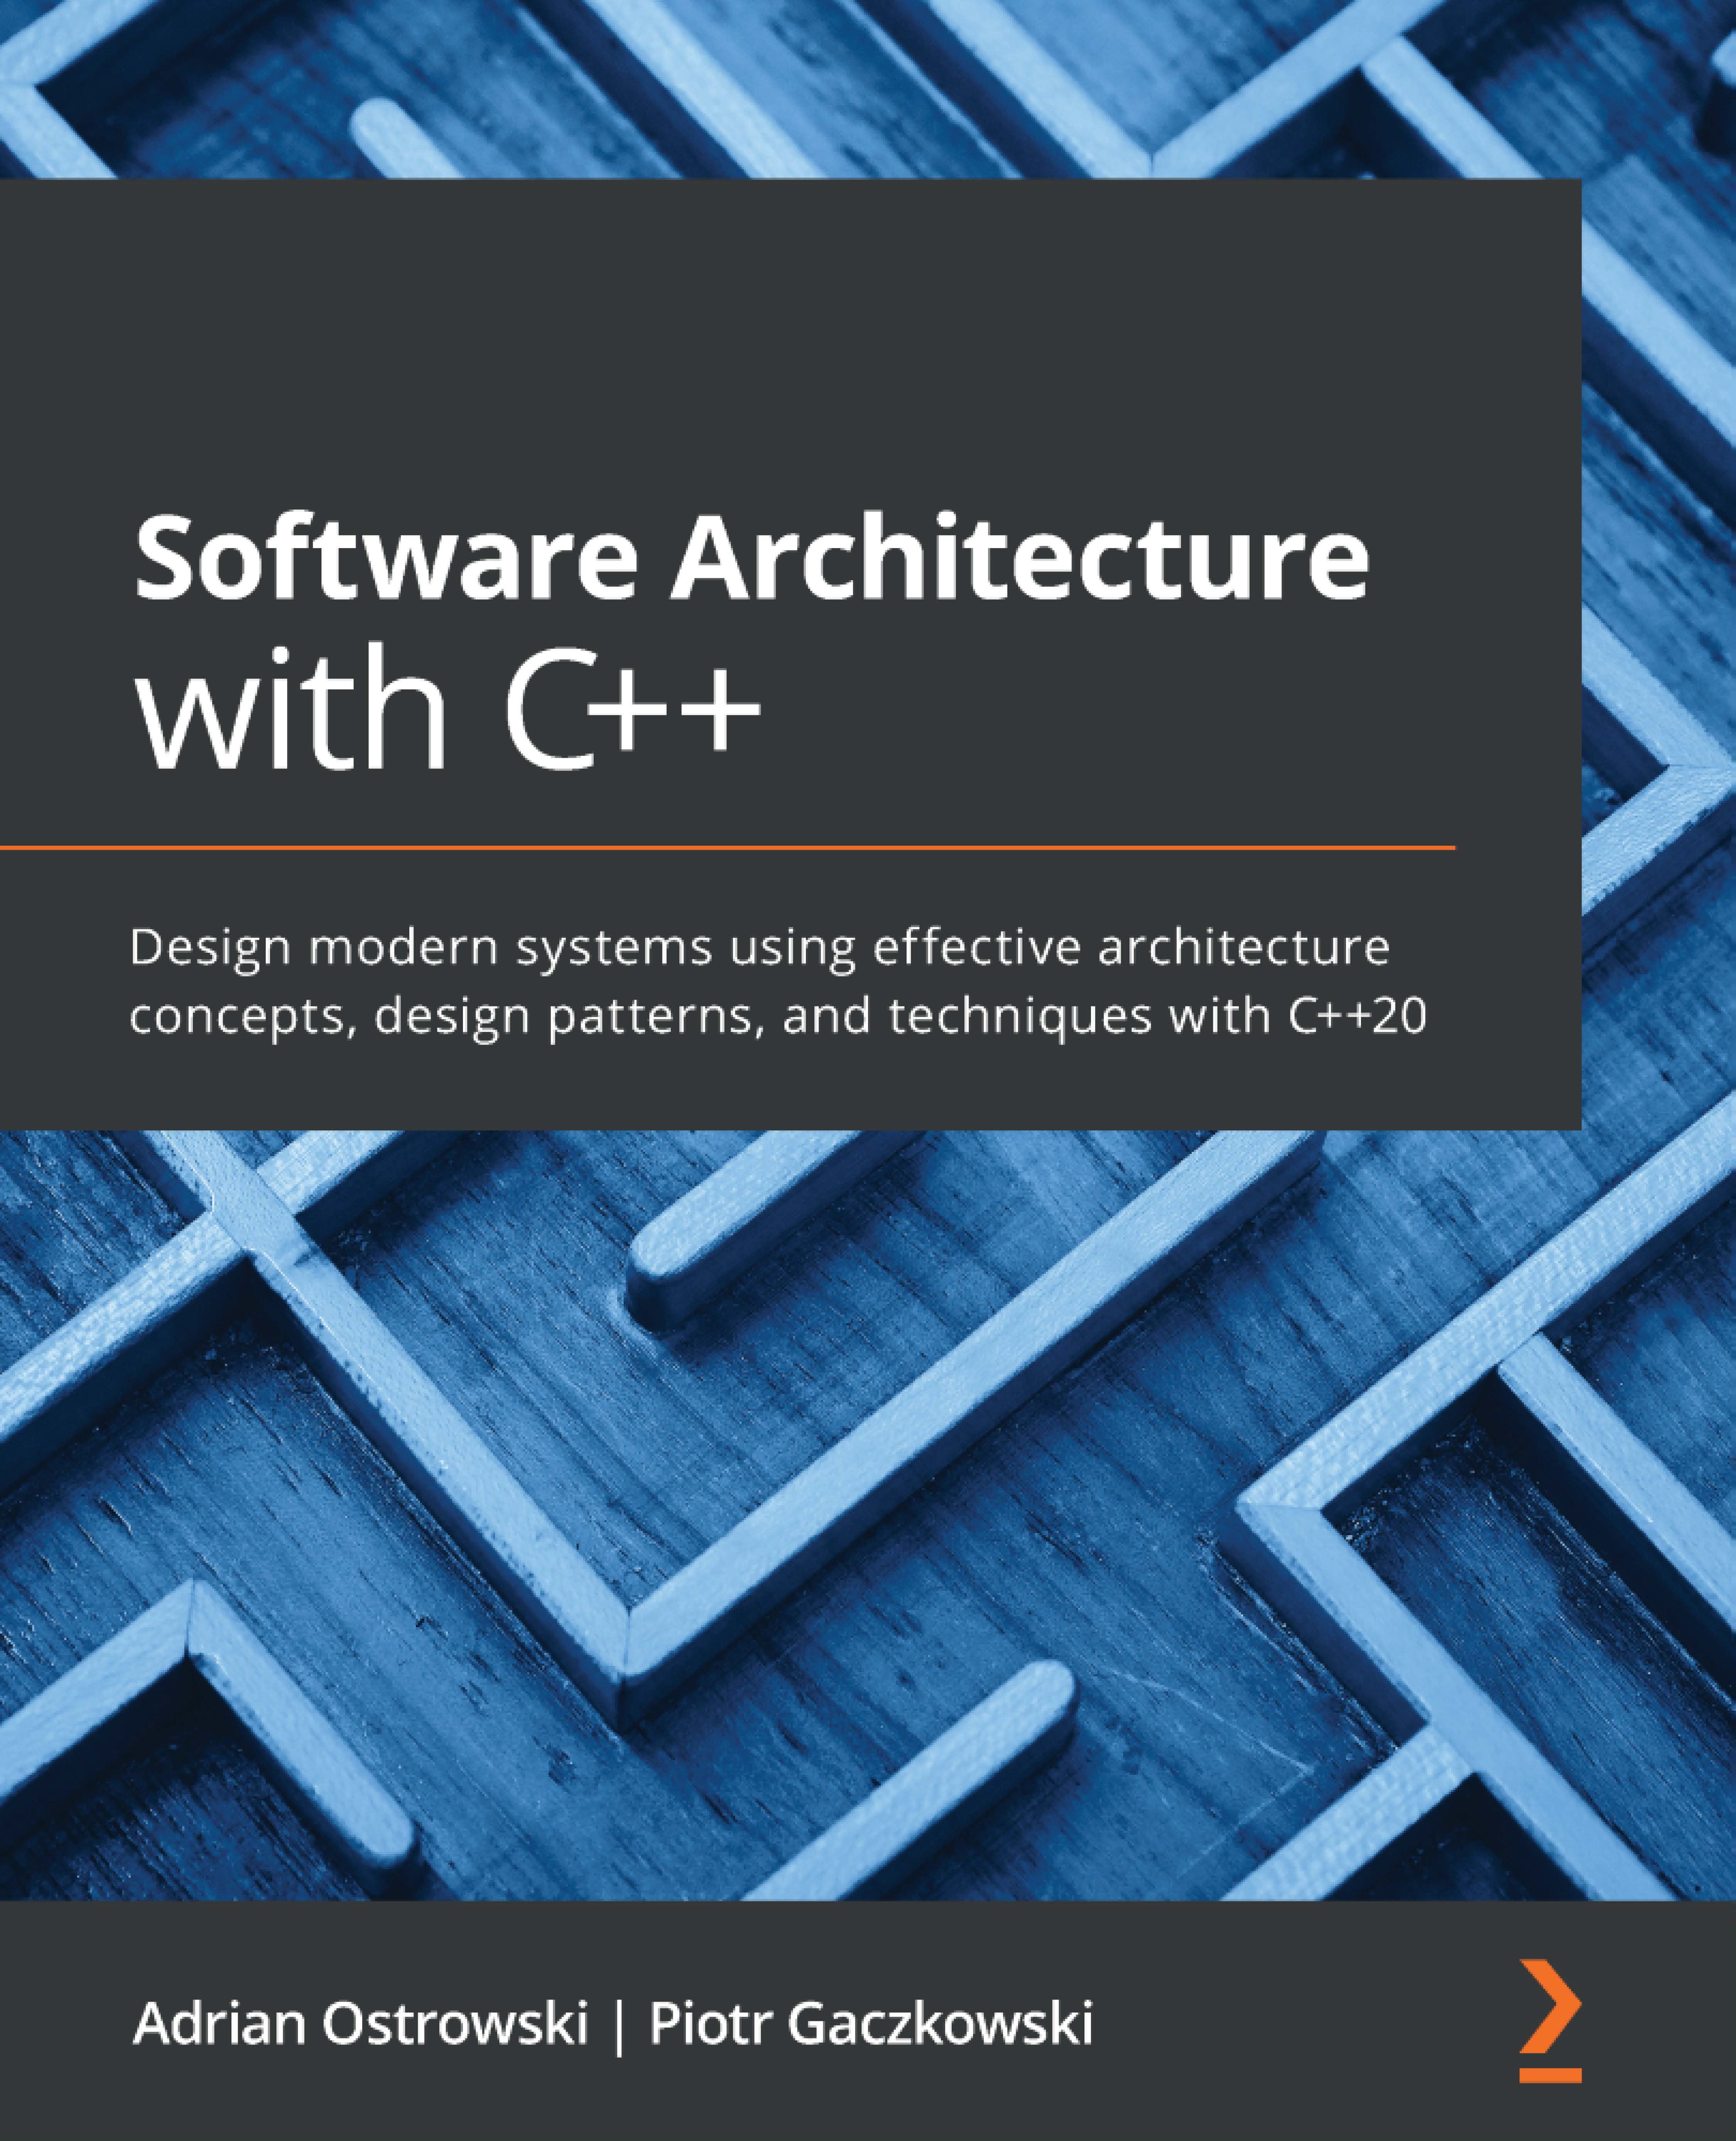
\includegraphics[width=\textwidth,height=\textheight,keepaspectratio]{cover.jpg}
\begin{tikzpicture}[remember picture, overlay, inner sep=0pt]
	\node at (current page.center) 
	{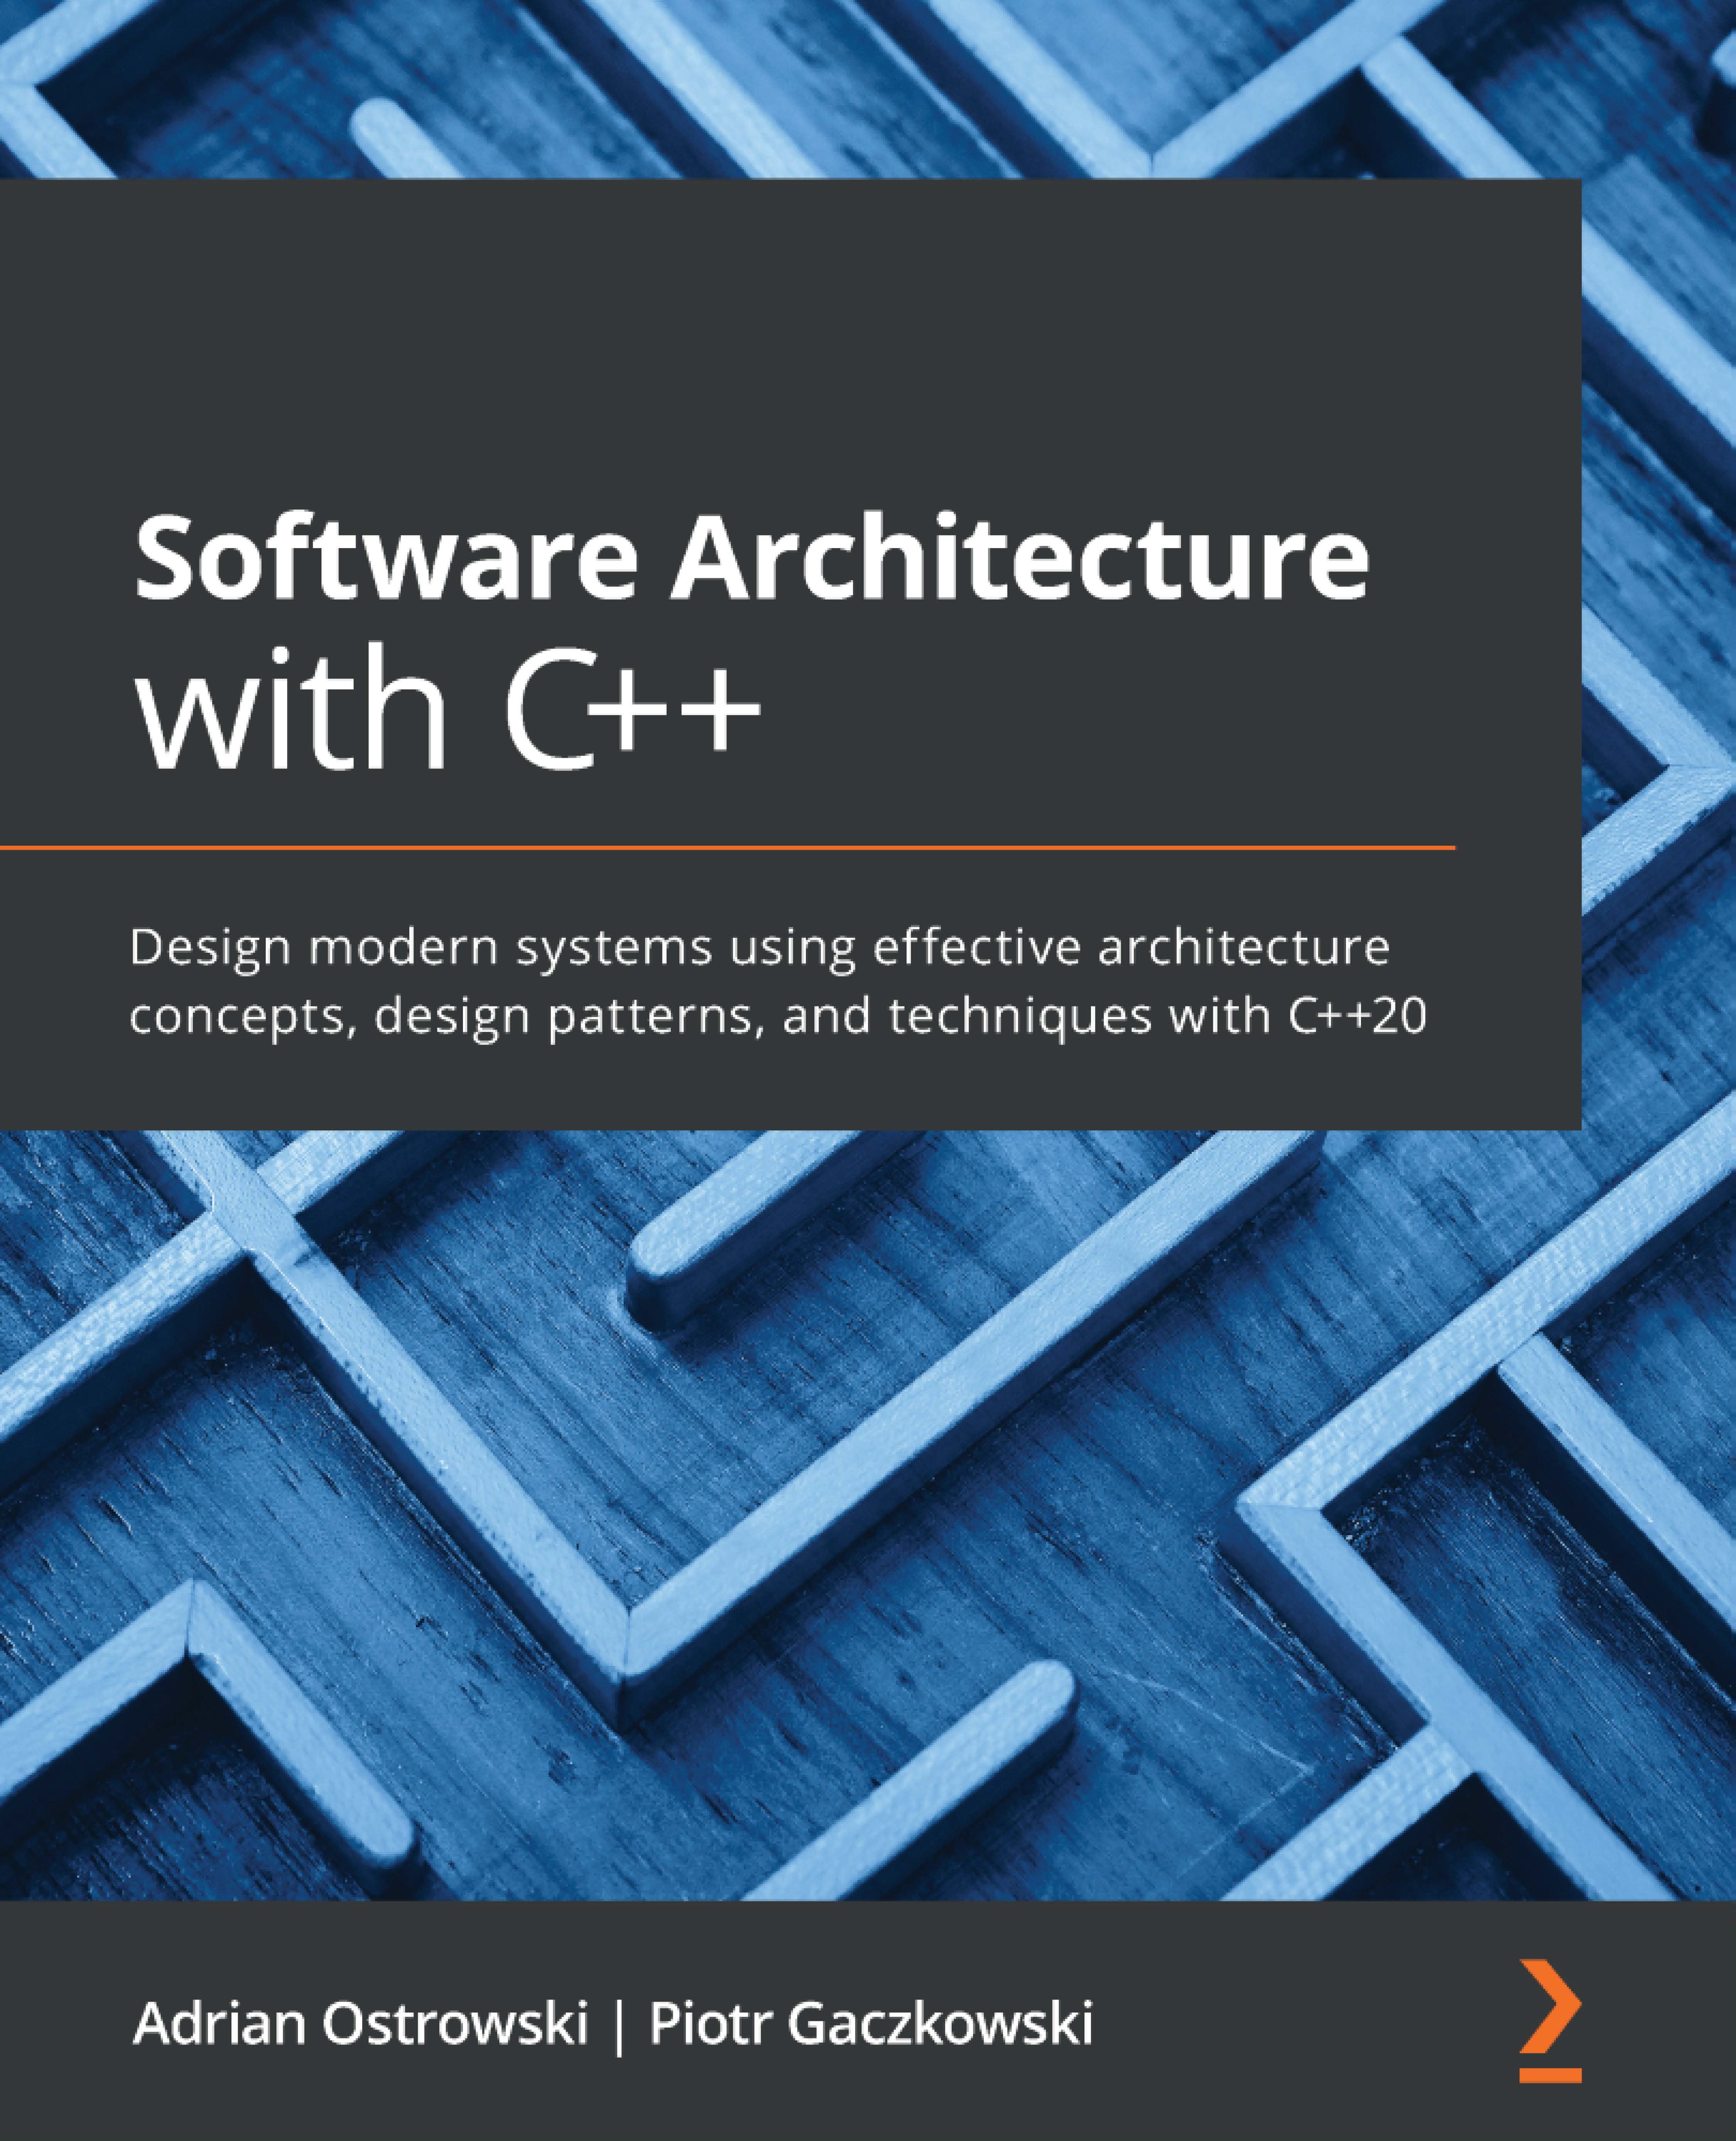
\includegraphics[width=\paperwidth, keepaspectratio=false]{cover.jpg}};
\end{tikzpicture}
\newpage
\thispagestyle{empty}
\huge
\textbf{The Art of Writing Efficient Programs} 
\\[9pt]
\normalsize
An advanced programmer's guide to efficient hardware utilization and compiler optimizations using C++ examples \\ 
(一本高級編程指南,使用C++介紹如何高效利用硬件和編譯器優化)
\\[10pt]
\normalsize 
作者: Fedor G. Pikus
\\[8pt]
\normalsize
譯者;陳曉偉
\end{center}

\hspace*{\fill} \\ %插入空行
\noindent\textbf{本書概述}

\textit{掌握各種性能提升技術,如併發性、無鎖編程、原子操作、並行性和內存管理。}

性能自提升的時代結束了,以前隨著CPU的升級,程序本身的速度也在加快,現在情況不一樣了。新架構的處理器時鐘頻率幾乎達到了峰值,對現有的程序性能上的改進並不多。雖然處理器的體積更大、性能更強,但這些能力的都在增多的核數和其他的計算單元上消耗掉了。為了編寫高效的軟件,現在的開發者必須瞭解如何利用現有的計算資源進行編程,這本書將說明如何做到這一點。

這本書涵蓋了編寫高效程序的主要方面:高效地使用CPU資源和內存,避免不必要的計算,性能測試,以及如何充分利用併發性和多線程。還會了解編譯器優化,以及如何更有效地使用編程語言(C++)。最後,瞭解設計決策如何對性能產生影響。

讀完這本書,可以利用處理器和編譯器的知識來編寫高效的程序,還能夠理解使用這些技術和在提高性能時如何進行測試。而本書的核心在於學習的方法論。

\hspace*{\fill} \\ %插入空行
\noindent\textbf{關鍵特性}
\begin{itemize}
\item 瞭解現代CPU的侷限性及對性能的影響
\item 瞭解如何避免編寫效率低下的代碼,並使用編譯器進行優化
\item 瞭解編寫高性能程序需要權衡策略和成本
\end{itemize}

\hspace*{\fill} \\ %插入空行
\noindent\textbf{內容綱要}
\begin{itemize}
\item 瞭解如何有效地使用程序中的硬件計算資源
\item 理解內存序和內存柵欄之間的關係
\item 熟悉不同數據結構和組織方式對性能的影響
\item 評估併發內存訪問對性能的影響,以及如何將影響最小化
\item 瞭解何時使用和不使用無鎖編程技術
\item 探索提高編譯器優化效率的不同方法
\item 為避免效率低下的開發,針對併發和高性能數據結構設計API
\end{itemize}

\hspace*{\fill} \\ %插入空行
\noindent\textbf{作者簡介}

\textbf{Fedor G. Pikus}是Mentor Graphics公司(西門子公司)硅設計部門的首席工程科學家。他曾在谷歌擔任高級軟件工程師,在Mentor Graphics擔任Calibre PERC、LVS、DFM的首席軟件架構師。1998年,他從計算物理的學術研究轉向軟件行業,加入Mentor Graphics。Fedor是高性能計算和C++方面公認的專家,他的作品在CPPCon, SD West, DesignCon, Software Development Journal上進行過展示,也是O'Reilly的作者。作為首席科學家,他的職責包括規劃Calibre產品的長期技術方向,指導和培訓從事這些產品、軟件設計和架構的工程師,以及研究新的設計和軟件技術。Fedor在物理學、EDA、軟件設計和C++語言方面擁有超過25項專利和超過100篇論文和會議報告。
\begin{center}
\tt
我要感謝我的妻子加林娜(Galina),我的兒子亞倫(Aaron)和本傑明(Benjamin),他們支持和鼓勵我,對我信心十足。還有我的貓維尼(Pooh),也會在我需要的時候鼓勵我。
\end{center}

\thispagestyle{empty}
\hspace*{\fill} \\ %插入空行
\noindent\textbf{審評者介紹}

\textbf{Sergey Gomon}在12年前在白俄羅斯國立大學信息和無線電電子學院的人工智能系,開始了他的IT之旅。他在網絡編程、信息安全、圖像處理等多個領域擁有大約8年使用C++的工業編程經驗。他目前在N-able工作,是CoreHard C++社區的活躍成員。


\hspace*{\fill} \\ %插入空行
\noindent\textbf{本書相關}
\begin{itemize}
\item Github翻譯地址:\\\url{https://github.com/xiaoweiChen/The-Art-of-Writing-Efficient-Programs}
\end{itemize}
\newpage

%前言
\pagestyle{empty}
\subfile{content/preface.tex}

\tableofcontents
\newpage

\setsecnumdepth{section}

\color{white}
\section*{\zihao{1}第一部分:性能基礎}
\pagecolor{mygray}
\addcontentsline{toc}{section}{第一部分:性能基礎}
\textbf{\subfile{content/1/Section-1.tex}}
\newpage
\color{black}
\pagecolor{white}

\subsection*{\zihao{2} 第1章\hspace{0.5cm}性能和併發性}
\addcontentsline{toc}{subsection}{第1章\hspace{0.5cm}性能和併發性}
\subfile{content/1/chapter1/0.tex}

\subsubsection*{\zihao{3} 1.1.\hspace{0.2cm}為什麼要關注性能?}
\addcontentsline{toc}{subsubsection}{1.1.\hspace{0.2cm}為什麼要關注性能?}
\subfile{content/1/chapter1/1.tex}

\subsubsection*{\zihao{3} 1.2.\hspace{0.2cm}為什麼有性能問題}
\addcontentsline{toc}{subsubsection}{1.2.\hspace{0.2cm}為什麼有性能問題}
\subfile{content/1/chapter1/2.tex}

\subsubsection*{\zihao{3} 1.3.\hspace{0.2cm}性能是什麼?}
\addcontentsline{toc}{subsubsection}{1.3.\hspace{0.2cm}性能是什麼?}
\subfile{content/1/chapter1/3.tex}

\subsubsection*{\zihao{3} 1.4.\hspace{0.2cm}評估、估計和預測性能}
\addcontentsline{toc}{subsubsection}{1.4.\hspace{0.2cm}評估、估計和預測性能}
\subfile{content/1/chapter1/4.tex}

\subsubsection*{\zihao{3} 1.5.\hspace{0.2cm}高性能}
\addcontentsline{toc}{subsubsection}{1.5.\hspace{0.2cm}高性能}
\subfile{content/1/chapter1/5.tex}

\subsubsection*{\zihao{3} 1.6.\hspace{0.2cm}總結}
\addcontentsline{toc}{subsubsection}{1.6.\hspace{0.2cm}總結}
\subfile{content/1/chapter1/6.tex}

\subsubsection*{\zihao{3} 1.7.\hspace{0.2cm}練習題}
\addcontentsline{toc}{subsubsection}{1.7.\hspace{0.2cm}練習題}
\subfile{content/1/chapter1/7.tex}
\newpage

\subsection*{\zihao{2} 第2章\hspace{0.5cm}性能測試}
\addcontentsline{toc}{subsection}{第2章\hspace{0.5cm}性能測試}
\subfile{content/1/chapter2/0.tex}

\subsubsection*{\zihao{3} 2.1.\hspace{0.2cm}相關準備}
\addcontentsline{toc}{subsubsection}{2.1.\hspace{0.2cm}相關準備}
\subfile{content/1/chapter2/1.tex}

\subsubsection*{\zihao{3} 2.2.\hspace{0.2cm}性能測試示例}
\addcontentsline{toc}{subsubsection}{2.2.\hspace{0.2cm}性能測試示例}
\subfile{content/1/chapter2/2.tex}

\subsubsection*{\zihao{3} 2.3.\hspace{0.2cm}性能基準測試}
\addcontentsline{toc}{subsubsection}{2.3.\hspace{0.2cm}性能基準測試}
\subfile{content/1/chapter2/3.tex}

\subsubsection*{\zihao{3} 2.4.\hspace{0.2cm}性能分析}
\addcontentsline{toc}{subsubsection}{2.4.\hspace{0.2cm}性能分析}
\subfile{content/1/chapter2/4.tex}

\subsubsection*{\zihao{3} 2.5.\hspace{0.2cm}微基準測試}
\addcontentsline{toc}{subsubsection}{2.5.\hspace{0.2cm}微基準測試}
\subfile{content/1/chapter2/5.tex}

\subsubsection*{\zihao{3} 2.6.\hspace{0.2cm}總結}
\addcontentsline{toc}{subsubsection}{2.6.\hspace{0.2cm}總結}
\subfile{content/1/chapter2/6.tex}

\subsubsection*{\zihao{3} 2.7.\hspace{0.2cm}練習題}
\addcontentsline{toc}{subsubsection}{2.7.\hspace{0.2cm}練習題}
\subfile{content/1/chapter2/7.tex}
\newpage

\subsection*{\zihao{2} 第3章\hspace{0.5cm}CPU架構、資源和性能}
\addcontentsline{toc}{subsection}{第3章\hspace{0.5cm}CPU架構、資源和性能}
\subfile{content/1/chapter3/0.tex}

\subsubsection*{\zihao{3} 3.1.\hspace{0.2cm}相關準備}
\addcontentsline{toc}{subsubsection}{3.1.\hspace{0.2cm}相關準備}
\subfile{content/1/chapter3/1.tex}

\subsubsection*{\zihao{3} 3.2.\hspace{0.2cm}從CPU性能開始}
\addcontentsline{toc}{subsubsection}{3.2.\hspace{0.2cm}從CPU性能開始}
\subfile{content/1/chapter3/2.tex}

\subsubsection*{\zihao{3} 3.3.\hspace{0.2cm}微基準測試性能}
\addcontentsline{toc}{subsubsection}{3.3.\hspace{0.2cm}微基準測試性能}
\subfile{content/1/chapter3/3.tex}

\subsubsection*{\zihao{3} 3.4.\hspace{0.2cm}數據依賴和流水線}
\addcontentsline{toc}{subsubsection}{3.4.\hspace{0.2cm}數據依賴和流水線}
\subfile{content/1/chapter3/4.tex}

\subsubsection*{\zihao{3} 3.5.\hspace{0.2cm}流水線和分支}
\addcontentsline{toc}{subsubsection}{3.5.\hspace{0.2cm}流水線和分支}
\subfile{content/1/chapter3/5.tex}

\subsubsection*{\zihao{3} 3.6.\hspace{0.2cm}投機執行}
\addcontentsline{toc}{subsubsection}{3.6.\hspace{0.2cm}投機執行}
\subfile{content/1/chapter3/6.tex}

\subsubsection*{\zihao{3} 3.7.\hspace{0.2cm}複雜條件的優化}
\addcontentsline{toc}{subsubsection}{3.7.\hspace{0.2cm}複雜條件的優化}
\subfile{content/1/chapter3/7.tex}

\subsubsection*{\zihao{3} 3.8.\hspace{0.2cm}無分支計算}
\addcontentsline{toc}{subsubsection}{3.8.\hspace{0.2cm}無分支計算}
\subfile{content/1/chapter3/8.tex}

\subsubsection*{\zihao{3} 3.9.\hspace{0.2cm}總結}
\addcontentsline{toc}{subsubsection}{3.9.\hspace{0.2cm}總結}
\subfile{content/1/chapter3/9.tex}

\subsubsection*{\zihao{3} 3.10.\hspace{0.2cm}練習題}
\addcontentsline{toc}{subsubsection}{3.10.\hspace{0.2cm}練習題}
\subfile{content/1/chapter3/10.tex}
\newpage

\subsection*{\zihao{2} 第4章\hspace{0.5cm}內存架構與性能}
\addcontentsline{toc}{subsection}{第4章\hspace{0.5cm}內存架構與性能}
\subfile{content/1/chapter4/0.tex}

\subsubsection*{\zihao{3} 4.1.\hspace{0.2cm}相關準備}
\addcontentsline{toc}{subsubsection}{4.1.\hspace{0.2cm}相關準備}
\subfile{content/1/chapter4/1.tex}

\subsubsection*{\zihao{3} 4.2.\hspace{0.2cm}性能從CPU開始,但不會到此為止}
\addcontentsline{toc}{subsubsection}{4.2.\hspace{0.2cm}性能從CPU開始,但不會到此為止}
\subfile{content/1/chapter4/2.tex}

\subsubsection*{\zihao{3} 4.3.\hspace{0.2cm}測試訪問存速度}
\addcontentsline{toc}{subsubsection}{4.3.\hspace{0.2cm}測試訪問存速度}
\subfile{content/1/chapter4/3.tex}

\subsubsection*{\zihao{3} 4.4.\hspace{0.2cm}內存速度:數字}
\addcontentsline{toc}{subsubsection}{4.4.\hspace{0.2cm}內存速度:數字}
\subfile{content/1/chapter4/4.tex}

\subsubsection*{\zihao{3} 4.5.\hspace{0.2cm}優化內存性能}
\addcontentsline{toc}{subsubsection}{4.5.\hspace{0.2cm}優化內存性能}
\subfile{content/1/chapter4/5.tex}

\subsubsection*{\zihao{3} 4.6.\hspace{0.2cm}機器裡的幽靈}
\addcontentsline{toc}{subsubsection}{4.6.\hspace{0.2cm}機器裡的幽靈}
\subfile{content/1/chapter4/6.tex}

\subsubsection*{\zihao{3} 4.7.\hspace{0.2cm}總結}
\addcontentsline{toc}{subsubsection}{4.7.\hspace{0.2cm}總結}
\subfile{content/1/chapter4/7.tex}

\subsubsection*{\zihao{3} 4.8.\hspace{0.2cm}練習題}
\addcontentsline{toc}{subsubsection}{4.8.\hspace{0.2cm}練習題}
\subfile{content/1/chapter4/8.tex}
\newpage

\subsection*{\zihao{2} 第5章\hspace{0.5cm}線程、內存和併發}
\addcontentsline{toc}{subsection}{第5章\hspace{0.5cm}線程、內存和併發}
\subfile{content/1/chapter5/0.tex}

\subsubsection*{\zihao{3} 5.1.\hspace{0.2cm}相關準備}
\addcontentsline{toc}{subsubsection}{5.1.\hspace{0.2cm}相關準備}
\subfile{content/1/chapter5/1.tex}

\subsubsection*{\zihao{3} 5.2.\hspace{0.2cm}線程和併發}
\addcontentsline{toc}{subsubsection}{5.2.\hspace{0.2cm}線程和併發}
\subfile{content/1/chapter5/2.tex}

\subsubsection*{\zihao{3} 5.3.\hspace{0.2cm}內存同步的代價}
\addcontentsline{toc}{subsubsection}{5.3.\hspace{0.2cm}內存同步的代價}
\subfile{content/1/chapter5/3.tex}

\subsubsection*{\zihao{3} 5.4.\hspace{0.2cm}數據共享很貴}
\addcontentsline{toc}{subsubsection}{5.4.\hspace{0.2cm}數據共享很貴}
\subfile{content/1/chapter5/4.tex}

\subsubsection*{\zihao{3} 5.5.\hspace{0.2cm}併發和內存序}
\addcontentsline{toc}{subsubsection}{5.5.\hspace{0.2cm}併發和內存序}
\subfile{content/1/chapter5/5.tex}

\subsubsection*{\zihao{3} 5.6.\hspace{0.2cm}內存模型}
\addcontentsline{toc}{subsubsection}{5.6.\hspace{0.2cm}內存模型}
\subfile{content/1/chapter5/6.tex}

\subsubsection*{\zihao{3} 5.7.\hspace{0.2cm}總結}
\addcontentsline{toc}{subsubsection}{5.7.\hspace{0.2cm}總結}
\subfile{content/1/chapter5/7.tex}

\subsubsection*{\zihao{3} 5.8.\hspace{0.2cm}練習題}
\addcontentsline{toc}{subsubsection}{5.8.\hspace{0.2cm}練習題}
\subfile{content/1/chapter5/8.tex}
\newpage

\color{white}
\section*{\zihao{1}第二部分:高級併發}
\pagecolor{mygray}
\addcontentsline{toc}{section}{第二部分:高級併發}
\textbf{\subfile{content/2/Section-2.tex}}
\newpage
\color{black}
\pagecolor{white}

\subsection*{\zihao{2} 第6章\hspace{0.5cm}併發性和性能}
\addcontentsline{toc}{subsection}{第6章\hspace{0.5cm}併發性和性能}
\subfile{content/2/chapter6/0.tex}

\subsubsection*{\zihao{3} 6.1.\hspace{0.2cm}相關準備}
\addcontentsline{toc}{subsubsection}{6.1.\hspace{0.2cm}相關準備}
\subfile{content/2/chapter6/1.tex}

\subsubsection*{\zihao{3} 6.2.\hspace{0.2cm}如何高效地使用併發?}
\addcontentsline{toc}{subsubsection}{6.2.\hspace{0.2cm}如何高效地使用併發?}
\subfile{content/2/chapter6/2.tex}

\subsubsection*{\zihao{3} 6.3.\hspace{0.2cm}鎖的替代方案以及性能}
\addcontentsline{toc}{subsubsection}{6.3.\hspace{0.2cm}鎖的替代方案以及性能}
\subfile{content/2/chapter6/3.tex}

\subsubsection*{\zihao{3} 6.4.\hspace{0.2cm}併發編程的構建塊}
\addcontentsline{toc}{subsubsection}{6.4.\hspace{0.2cm}併發編程的構建塊}
\subfile{content/2/chapter6/4.tex}

\subsubsection*{\zihao{3} 6.5.\hspace{0.2cm}總結}
\addcontentsline{toc}{subsubsection}{6.5.\hspace{0.2cm}總結}
\subfile{content/2/chapter6/5.tex}

\subsubsection*{\zihao{3} 6.6.\hspace{0.2cm}練習題}
\addcontentsline{toc}{subsubsection}{6.6.\hspace{0.2cm}練習題}
\subfile{content/2/chapter6/6.tex}
\newpage

\subsection*{\zihao{2} 第7章\hspace{0.5cm}用於併發的數據結構}
\addcontentsline{toc}{subsection}{第7章\hspace{0.5cm}用於併發的數據結構}
\subfile{content/2/chapter7/0.tex}

\subsubsection*{\zihao{3} 7.1.\hspace{0.2cm}相關準備}
\addcontentsline{toc}{subsubsection}{7.1.\hspace{0.2cm}相關準備}
\subfile{content/2/chapter7/1.tex}

\subsubsection*{\zihao{3} 7.2.\hspace{0.2cm}線程安全的數據結構}
\addcontentsline{toc}{subsubsection}{7.2.\hspace{0.2cm}線程安全的數據結構}
\subfile{content/2/chapter7/2.tex}

\subsubsection*{\zihao{3} 7.3.\hspace{0.2cm}線程安全的堆棧}
\addcontentsline{toc}{subsubsection}{7.3.\hspace{0.2cm}線程安全的堆棧}
\subfile{content/2/chapter7/3.tex}

\subsubsection*{\zihao{3} 7.4.\hspace{0.2cm}線程安全的隊列}
\addcontentsline{toc}{subsubsection}{7.4.\hspace{0.2cm}線程安全的隊列}
\subfile{content/2/chapter7/4.tex}

\subsubsection*{\zihao{3} 7.5.\hspace{0.2cm}線程安全的鏈表}
\addcontentsline{toc}{subsubsection}{7.5.\hspace{0.2cm}線程安全的鏈表}
\subfile{content/2/chapter7/5.tex}

\subsubsection*{\zihao{3} 7.6.\hspace{0.2cm}總結}
\addcontentsline{toc}{subsubsection}{7.6.\hspace{0.2cm}總結}
\subfile{content/2/chapter7/6.tex}

\subsubsection*{\zihao{3} 7.7.\hspace{0.2cm}練習題}
\addcontentsline{toc}{subsubsection}{7.7.\hspace{0.2cm}練習題}
\subfile{content/2/chapter7/7.tex}
\newpage

\subsection*{\zihao{2} 第8章\hspace{0.5cm}C++中的併發}
\addcontentsline{toc}{subsection}{第8章\hspace{0.5cm}C++中的併發}
\subfile{content/2/chapter8/0.tex}

\subsubsection*{\zihao{3} 8.1.\hspace{0.2cm}相關準備}
\addcontentsline{toc}{subsubsection}{8.1.\hspace{0.2cm}相關準備}
\subfile{content/2/chapter8/1.tex}

\subsubsection*{\zihao{3} 8.2.\hspace{0.2cm}C++11的併發支持}
\addcontentsline{toc}{subsubsection}{8.2.\hspace{0.2cm}C++11的併發支持}
\subfile{content/2/chapter8/2.tex}

\subsubsection*{\zihao{3} 8.3.\hspace{0.2cm}C++17的併發支持}
\addcontentsline{toc}{subsubsection}{8.3.\hspace{0.2cm}C++17的併發支持}
\subfile{content/2/chapter8/3.tex}

\subsubsection*{\zihao{3} 8.4.\hspace{0.2cm}C++20的併發支持}
\addcontentsline{toc}{subsubsection}{8.4.\hspace{0.2cm}C++20的併發支持}
\subfile{content/2/chapter8/4.tex}

\subsubsection*{\zihao{3} 8.5.\hspace{0.2cm}總結}
\addcontentsline{toc}{subsubsection}{8.5.\hspace{0.2cm}總結}
\subfile{content/2/chapter8/5.tex}

\subsubsection*{\zihao{3} 8.6.\hspace{0.2cm}練習題}
\addcontentsline{toc}{subsubsection}{8.6.\hspace{0.2cm}練習題}
\subfile{content/2/chapter8/6.tex}
\newpage

\color{white}
\section*{\zihao{1}第三部分:設計和編寫高性能程序}
\pagecolor{mygray}
\addcontentsline{toc}{section}{第三部分:設計和編寫高性能程序}
\textbf{\subfile{content/3/Section-3.tex}}
\newpage
\color{black}
\pagecolor{white}

\subsection*{\zihao{2} 第9章\hspace{0.5cm}高性能C++}
\addcontentsline{toc}{subsection}{第9章\hspace{0.5cm}高性能C++}
\subfile{content/3/chapter9/0.tex}

\subsubsection*{\zihao{3} 9.1.\hspace{0.2cm}相關準備}
\addcontentsline{toc}{subsubsection}{9.1.\hspace{0.2cm}相關準備}
\subfile{content/3/chapter9/1.tex}

\subsubsection*{\zihao{3} 9.2.\hspace{0.2cm}編程語言的效率}
\addcontentsline{toc}{subsubsection}{9.2.\hspace{0.2cm}編程語言的效率}
\subfile{content/3/chapter9/2.tex}

\subsubsection*{\zihao{3} 9.3.\hspace{0.2cm}不必要的複製}
\addcontentsline{toc}{subsubsection}{9.3.\hspace{0.2cm}不必要的複製}	
\subfile{content/3/chapter9/3.tex}

\subsubsection*{\zihao{3} 9.4.\hspace{0.2cm}低效的內存管理}
\addcontentsline{toc}{subsubsection}{9.4.\hspace{0.2cm}低效的內存管理}
\subfile{content/3/chapter9/4.tex}

\subsubsection*{\zihao{3} 9.5.\hspace{0.2cm}條件執行的優化}
\addcontentsline{toc}{subsubsection}{9.5.\hspace{0.2cm}條件執行的優化}
\subfile{content/3/chapter9/5.tex}

\subsubsection*{\zihao{3} 9.6.\hspace{0.2cm}總結}
\addcontentsline{toc}{subsubsection}{9.6.\hspace{0.2cm}總結}
\subfile{content/3/chapter9/6.tex}

\subsubsection*{\zihao{3} 9.7.\hspace{0.2cm}練習題}
\addcontentsline{toc}{subsubsection}{9.7.\hspace{0.2cm}練習題}
\subfile{content/3/chapter9/7.tex}
\newpage

\subsection*{\zihao{2} 第10章\hspace{0.5cm}C++中的編譯器優化}
\addcontentsline{toc}{subsection}{第10章\hspace{0.5cm}C++中的編譯器優化}
\subfile{content/3/chapter10/0.tex}

\subsubsection*{\zihao{3} 10.1.\hspace{0.2cm}相關準備}
\addcontentsline{toc}{subsubsection}{10.1.\hspace{0.2cm}相關準備}
\subfile{content/3/chapter10/1.tex}

\subsubsection*{\zihao{3} 10.2.\hspace{0.2cm}編譯器優化代碼}
\addcontentsline{toc}{subsubsection}{10.2.\hspace{0.2cm}編譯器優化代碼}
\subfile{content/3/chapter10/2.tex}

\subsubsection*{\zihao{3} 10.3.\hspace{0.2cm}總結}
\addcontentsline{toc}{subsubsection}{10.3.\hspace{0.2cm}總結}
\subfile{content/3/chapter10/3.tex}

\subsubsection*{\zihao{3} 10.4.\hspace{0.2cm}練習題}
\addcontentsline{toc}{subsubsection}{10.4.\hspace{0.2cm}練習題}
\subfile{content/3/chapter10/4.tex}
\newpage

\subsection*{\zihao{2} 第11章\hspace{0.5cm}未定義的行為和性能}
\addcontentsline{toc}{subsection}{第11章\hspace{0.5cm}未定義的行為和性能}
\subfile{content/3/chapter11/0.tex}

\subsubsection*{\zihao{3} 11.1.\hspace{0.2cm}相關準備}
\addcontentsline{toc}{subsubsection}{11.1.\hspace{0.2cm}相關準備}
\subfile{content/3/chapter11/1.tex}

\subsubsection*{\zihao{3} 11.2.\hspace{0.2cm}未定義行為}
\addcontentsline{toc}{subsubsection}{11.2.\hspace{0.2cm}未定義行為}
\subfile{content/3/chapter11/2.tex}

\subsubsection*{\zihao{3} 11.3.\hspace{0.2cm}為什麼會有未定義的行為?}
\addcontentsline{toc}{subsubsection}{11.3.\hspace{0.2cm}為什麼會有未定義的行為?}
\subfile{content/3/chapter11/3.tex}

\subsubsection*{\zihao{3} 11.4.\hspace{0.2cm}未定義的行為和C++優化}
\addcontentsline{toc}{subsubsection}{11.4.\hspace{0.2cm}未定義的行為和C++優化}
\subfile{content/3/chapter11/4.tex}

\subsubsection*{\zihao{3} 11.5.\hspace{0.2cm}使用未定義的行為進行高效的設計}
\addcontentsline{toc}{subsubsection}{11.5.\hspace{0.2cm}使用未定義的行為進行高效的設計}
\subfile{content/3/chapter11/5.tex}

\subsubsection*{\zihao{3} 11.6.\hspace{0.2cm}總結}
\addcontentsline{toc}{subsubsection}{11.6.\hspace{0.2cm}總結}
\subfile{content/3/chapter11/6.tex}

\subsubsection*{\zihao{3} 11.7.\hspace{0.2cm}練習題}
\addcontentsline{toc}{subsubsection}{11.7.\hspace{0.2cm}練習題}
\subfile{content/3/chapter11/7.tex}
\newpage

\subsection*{\zihao{2} 第12章\hspace{0.5cm}為性能而設計}
\addcontentsline{toc}{subsection}{第12章\hspace{0.5cm}為性能而設計}
\subfile{content/3/chapter12/0.tex}

\subsubsection*{\zihao{3} 12.1.\hspace{0.2cm}相關準備}
\addcontentsline{toc}{subsubsection}{12.1.\hspace{0.2cm}相關準備}
\subfile{content/3/chapter12/1.tex}

\subsubsection*{\zihao{3} 12.2.\hspace{0.2cm}設計與性能間的關係}
\addcontentsline{toc}{subsubsection}{12.2.\hspace{0.2cm}設計與性能間的關係}
\subfile{content/3/chapter12/2.tex}

\subsubsection*{\zihao{3} 12.3.\hspace{0.2cm}為性能設計}
\addcontentsline{toc}{subsubsection}{12.3.\hspace{0.2cm}為性能設計}
\subfile{content/3/chapter12/3.tex}

\subsubsection*{\zihao{3} 12.4.\hspace{0.2cm}API的設計考慮}
\addcontentsline{toc}{subsubsection}{12.4.\hspace{0.2cm}API的設計考慮}
\subfile{content/3/chapter12/4.tex}

\subsubsection*{\zihao{3} 12.5.\hspace{0.2cm}為最佳數據訪問而設計}
\addcontentsline{toc}{subsubsection}{12.5.\hspace{0.2cm}為最佳數據訪問而設計}
\subfile{content/3/chapter12/5.tex}

\subsubsection*{\zihao{3} 12.6.\hspace{0.2cm}性能的權衡}
\addcontentsline{toc}{subsubsection}{12.6.\hspace{0.2cm}性能的權衡}
\subfile{content/3/chapter12/6.tex}

\subsubsection*{\zihao{3} 12.7.\hspace{0.2cm}明智的設計決策}
\addcontentsline{toc}{subsubsection}{12.7.\hspace{0.2cm}明智的設計決策}
\subfile{content/3/chapter12/7.tex}

\subsubsection*{\zihao{3} 12.8.\hspace{0.2cm}總結}
\addcontentsline{toc}{subsubsection}{12.8.\hspace{0.2cm}總結}
\subfile{content/3/chapter12/8.tex}

\subsubsection*{\zihao{3} 12.9.\hspace{0.2cm}練習題}
\addcontentsline{toc}{subsubsection}{12.9.\hspace{0.2cm}練習題}
\subfile{content/3/chapter12/9.tex}
\newpage

\section*{\zihao{2} 練習答案}
\addcontentsline{toc}{section}{練習答案}

\subsection*{\zihao{2}第1章}
\addcontentsline{toc}{subsection}{第1章}
\subfile{content/Assessments/1.tex}

\subsection*{\zihao{2}第2章}
\addcontentsline{toc}{subsection}{第2章}
\subfile{content/Assessments/2.tex}

\subsection*{\zihao{2}第3章}
\addcontentsline{toc}{subsection}{第3章}
\subfile{content/Assessments/3.tex}

\subsection*{\zihao{2}第4章}
\addcontentsline{toc}{subsection}{第4章}
\subfile{content/Assessments/4.tex}

\subsection*{\zihao{2}第5章}
\addcontentsline{toc}{subsection}{第5章}
\subfile{content/Assessments/5.tex}

\subsection*{\zihao{2}第6章}
\addcontentsline{toc}{subsection}{第6章}
\subfile{content/Assessments/6.tex}

\subsection*{\zihao{2}第7章}
\addcontentsline{toc}{subsection}{第7章}
\subfile{content/Assessments/7.tex}

\subsection*{\zihao{2}第8章}
\addcontentsline{toc}{subsection}{第8章}
\subfile{content/Assessments/8.tex}

\subsection*{\zihao{2}第9章}
\addcontentsline{toc}{subsection}{第9章}
\subfile{content/Assessments/9.tex}

\subsection*{\zihao{2}第10章}
\addcontentsline{toc}{subsection}{第10章}
\subfile{content/Assessments/10.tex}

\subsection*{\zihao{2}第11章}
\addcontentsline{toc}{subsection}{第11章}
\subfile{content/Assessments/11.tex}

\subsection*{\zihao{2}第12章}
\addcontentsline{toc}{subsection}{第12章}
\subfile{content/Assessments/12.tex}
	
\end{document}

